\documentclass{llncs}

\usepackage{graphicx}
\usepackage[noend]{algpseudocode}
\usepackage{subcaption}
\usepackage{caption}
\usepackage{microtype}
\captionsetup{compatibility=false}
\graphicspath{ {imgs/} }

\pdfinfo{
/Title (A Composable Strategy for Shredded Document Reconstruction)
/Author (Razvan Ranca, Iain Murray)
/Keywords (shredded document, reconstruction, strip-cut, cross-cut, unshred, deshred)
}

\begin{document}

\title{A Composable Strategy for Shredded Document Reconstruction}

\author{Razvan Ranca \and Iain Murray}

\institute{School of Informatics, University of Edinburgh,\\
10 Crichton Street, Edinburgh, Scotland, United Kingdom\\
\email{ranca.razvan@gmail.com},
\email{i.murray@ed.ac.uk}
}

\maketitle              % typeset the title of the contribution

\begin{abstract}
The reconstruction of shredded documents is of interest in domains such as forensics, investigative sciences and  archaeology, and has therefore been approached in many different ways. This paper takes a step towards bridging the gap between previous, disparate, efforts by proposing a composable, probabilistic solution. The task is first divided into independent sub-problems, and novel approaches to several of these sub-problems are then presented. The theoretical properties and empirical performance of these novel approaches are shown to compare favourably to those of previously published methods.
\keywords{shredded document, strip-cut, cross-cut, unshred, deshred}
\end{abstract}

\section{Introduction}

The US Federal Trade Commission recommends the shredding of sensitive documents as a good protection method against becoming one of the millions of victims of identity theft\footnote{http://consumer.ftc.gov/features/feature-0014-identity-theft}. However, the successfully solved DARPA Shredder challenge\footnote{http://archive.darpa.mil/shredderchallenge/} and the appearance of commercial document reconstruction services\footnote{eg: http://www.unshredder.com/}, raises questions about the current security offered by the shredder. Further research in this area will benefit projects such as the ongoing effort to recover the shredded archives of the East German secret police, which consist of 16,000 bags of shredded documents. Since it took 3 dozen people 6 years to reconstruct 300 of these bags (\cite{P6}), at this rate, the project would require 11,520 person-years.

In this paper, we approach the unshredding challenge by splitting the problem into four independent sub-problems. A \emph{pre-processing} step transforms the noisy images of scanned shreds into uniform ``ideal shreds". A \emph{scoring function} looks at the potential match between every pair of ideal shreds and indicates the viability of that match. A \emph{search method} is then employed to find a placement of the ideal shreds in 2D space that obtains a good global score, where the global score is the sum of the local scores determined by each pair of neighbouring shreds. Finally, a \emph{user-interaction} step can be weaved in with any of the above as to help catch errors before they have a chance to propagate.

 In Sections 3 to 5, we will present: a novel, composable and probabilistic scoring function; an original, graph-inspired, search heuristic which balances speed and accuracy while achieving modularity; and a tractable up/down orientation detection method which can be used as part of the pre-processing step.

\section{Related Work}
Significant effort has been made towards finding a good search function. In \cite{P1} the authors show that the search is NP hard by reduction to the Travelling Salesman Problem. Prandtstetter (\cite{P2}) attempts an Integer Linear Programming solution which yields good results but is intractable for more than 150 shreds. In \cite{P3,P4}, good results are obtained by applying evolutionary algorithms to the problem. 

In contrast, relatively little progress has been made in developing the score function. In \cite{P7,P2,P1,P3,P4}, the authors settled on a formulation which selects a score based on a weighted difference of the adjacent pixels on either side of the proposed join (\cite{P7} provides a formal definition of this method). Sleit, Massad and Musaddaq (\cite{P5}) refine this formulation by placing an emphasis on black pixels, thus discounting the information content of white pixels. In \cite{P8}, the authors try a different approach, by employing optical character recognition techniques. Their method is however left as a proof-of-concept, since it is not integrated with a search function or evaluated against any other scoring methods.

Pre-processing can be split into several independent functions, which have been previously explored. Skeoch (\cite{P9}) shows how to extract the shreds from scanned input images via rectangle and polynomial fitting. The authors of \cite{P10} fix the skew of the extracted shreds by framing the issue as an optimisation problem and finding the best rotation angle for each shred. Up/down orientation of documents is explored in \cite{P12,P11} with good results, though the methods are only evaluated on full documents, not shreds.

Finally, user-interaction has been approached in many ways. For instance, in \cite{P10,P5}, the authors allow the users to mark correct and incorrect edges between successive runs of the search method, while in \cite{P14} the scoring function is influenced by the user drawing what the neighbour of a shred might look like.

\section{Probabilistic Score}
We propose a novel score function formulation, which uses a probabilistic model to directly estimate the likelihood of two edges matching. Employing a probabilistic model offers several advantages, such as an increase in robustness given by the ability to train the model on the given document shreds and an ease of composability with other models, which can be achieved by simply multiplying the different predicted probabilities and re-normalising the results.

We test this idea by implementing a basic probabilistic model, which is based on the conditional probability that a pixel is white or black given a few of its neighbouring pixels. Formally, given edge \emph{Et}, \emph{ProbScore} returns the best match for Et and the probability of that match. ProbScore is defined as:
\begin{algorithmic}
\Procedure {ProbScore}{$Et$}
  \State {Initialise $ps$} \Comment{\emph{probabilities of matches, initially all 1}}
  \ForAll{$Ex \in Edges$} 
    \ForAll {$pixel \in Ex$}
      \State $ps_{Ex} \gets ps_{Ex} * \Pr(pixel|Neighbours_{Et}^{pixel})$ 
    \EndFor
  \EndFor
  \State {Normalise $ps$} \Comment{\emph{probabilities must sum up to 1}}
  \State \textbf{return} $\arg\max ps$, $\max ps$
\EndProcedure
\end{algorithmic}

Empirical results show that this probabilistic score compares favourably to the most common scoring function used in literature (\cite{P7}), both on noise-less documents and on several noisy documents (see Figure \ref{fig:scoreComp}). Additionally, in order to showcase the benefits offered by the composable nature of ProbScore, we combine it with another probabilistic model called \emph{RowScore}. RowScore calculates the distance between rows of text in neighbouring shreds and applies a Gaussian model to this distance. Even such a simple probabilistic model gives ProbScore a small but consistent boost (see Figure \ref{fig:scoreComp}). In a similar way, ProbScore could be composed with more complex models, such as that proposed in \cite{P8}.
\begin{figure}[h]
    \setlength{\abovecaptionskip}{4pt plus 1.0pt minus 2.0pt}
    \centering
    \begin{subfigure}[b]{0.48\textwidth}
        \setlength{\abovecaptionskip}{1pt plus 1.0pt minus 2.0pt}
        \centering
        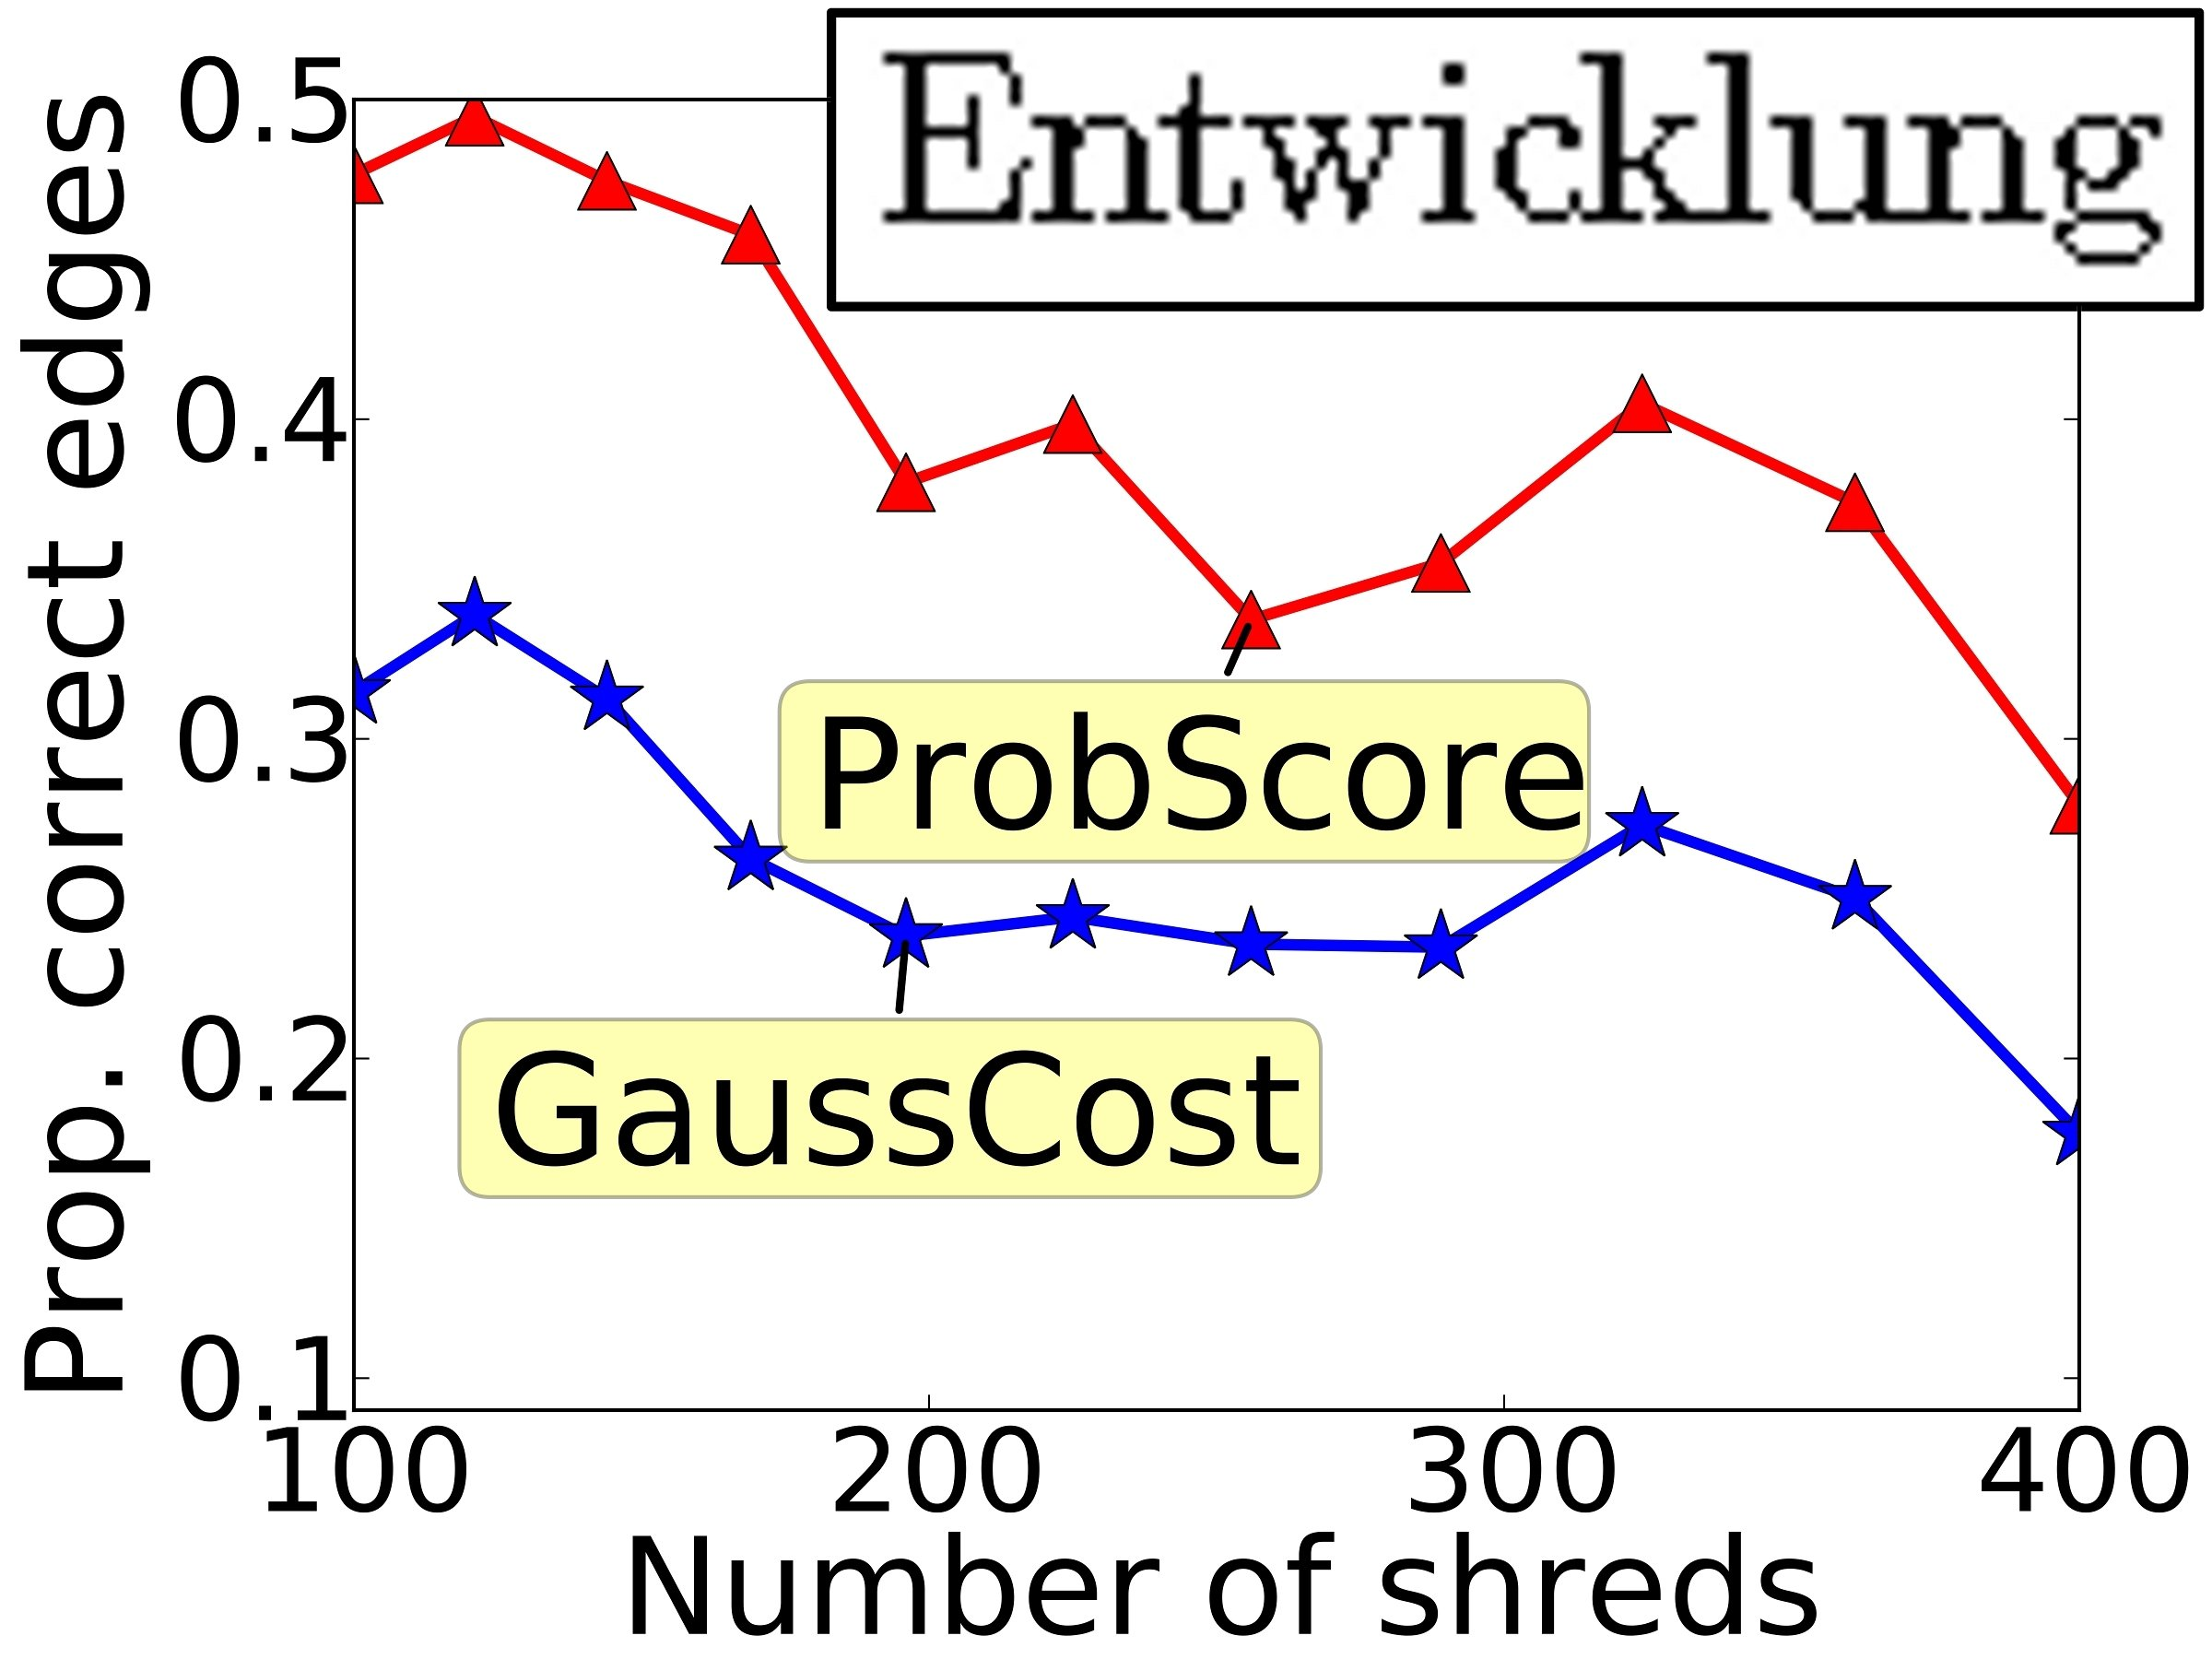
\includegraphics[width=\textwidth]{origCompEnt300.jpg}
        \caption{Original document.}
    \end{subfigure}
    \begin{subfigure}[b]{0.48\textwidth}
        \setlength{\abovecaptionskip}{1pt plus 1.0pt minus 2.0pt}
        \centering
        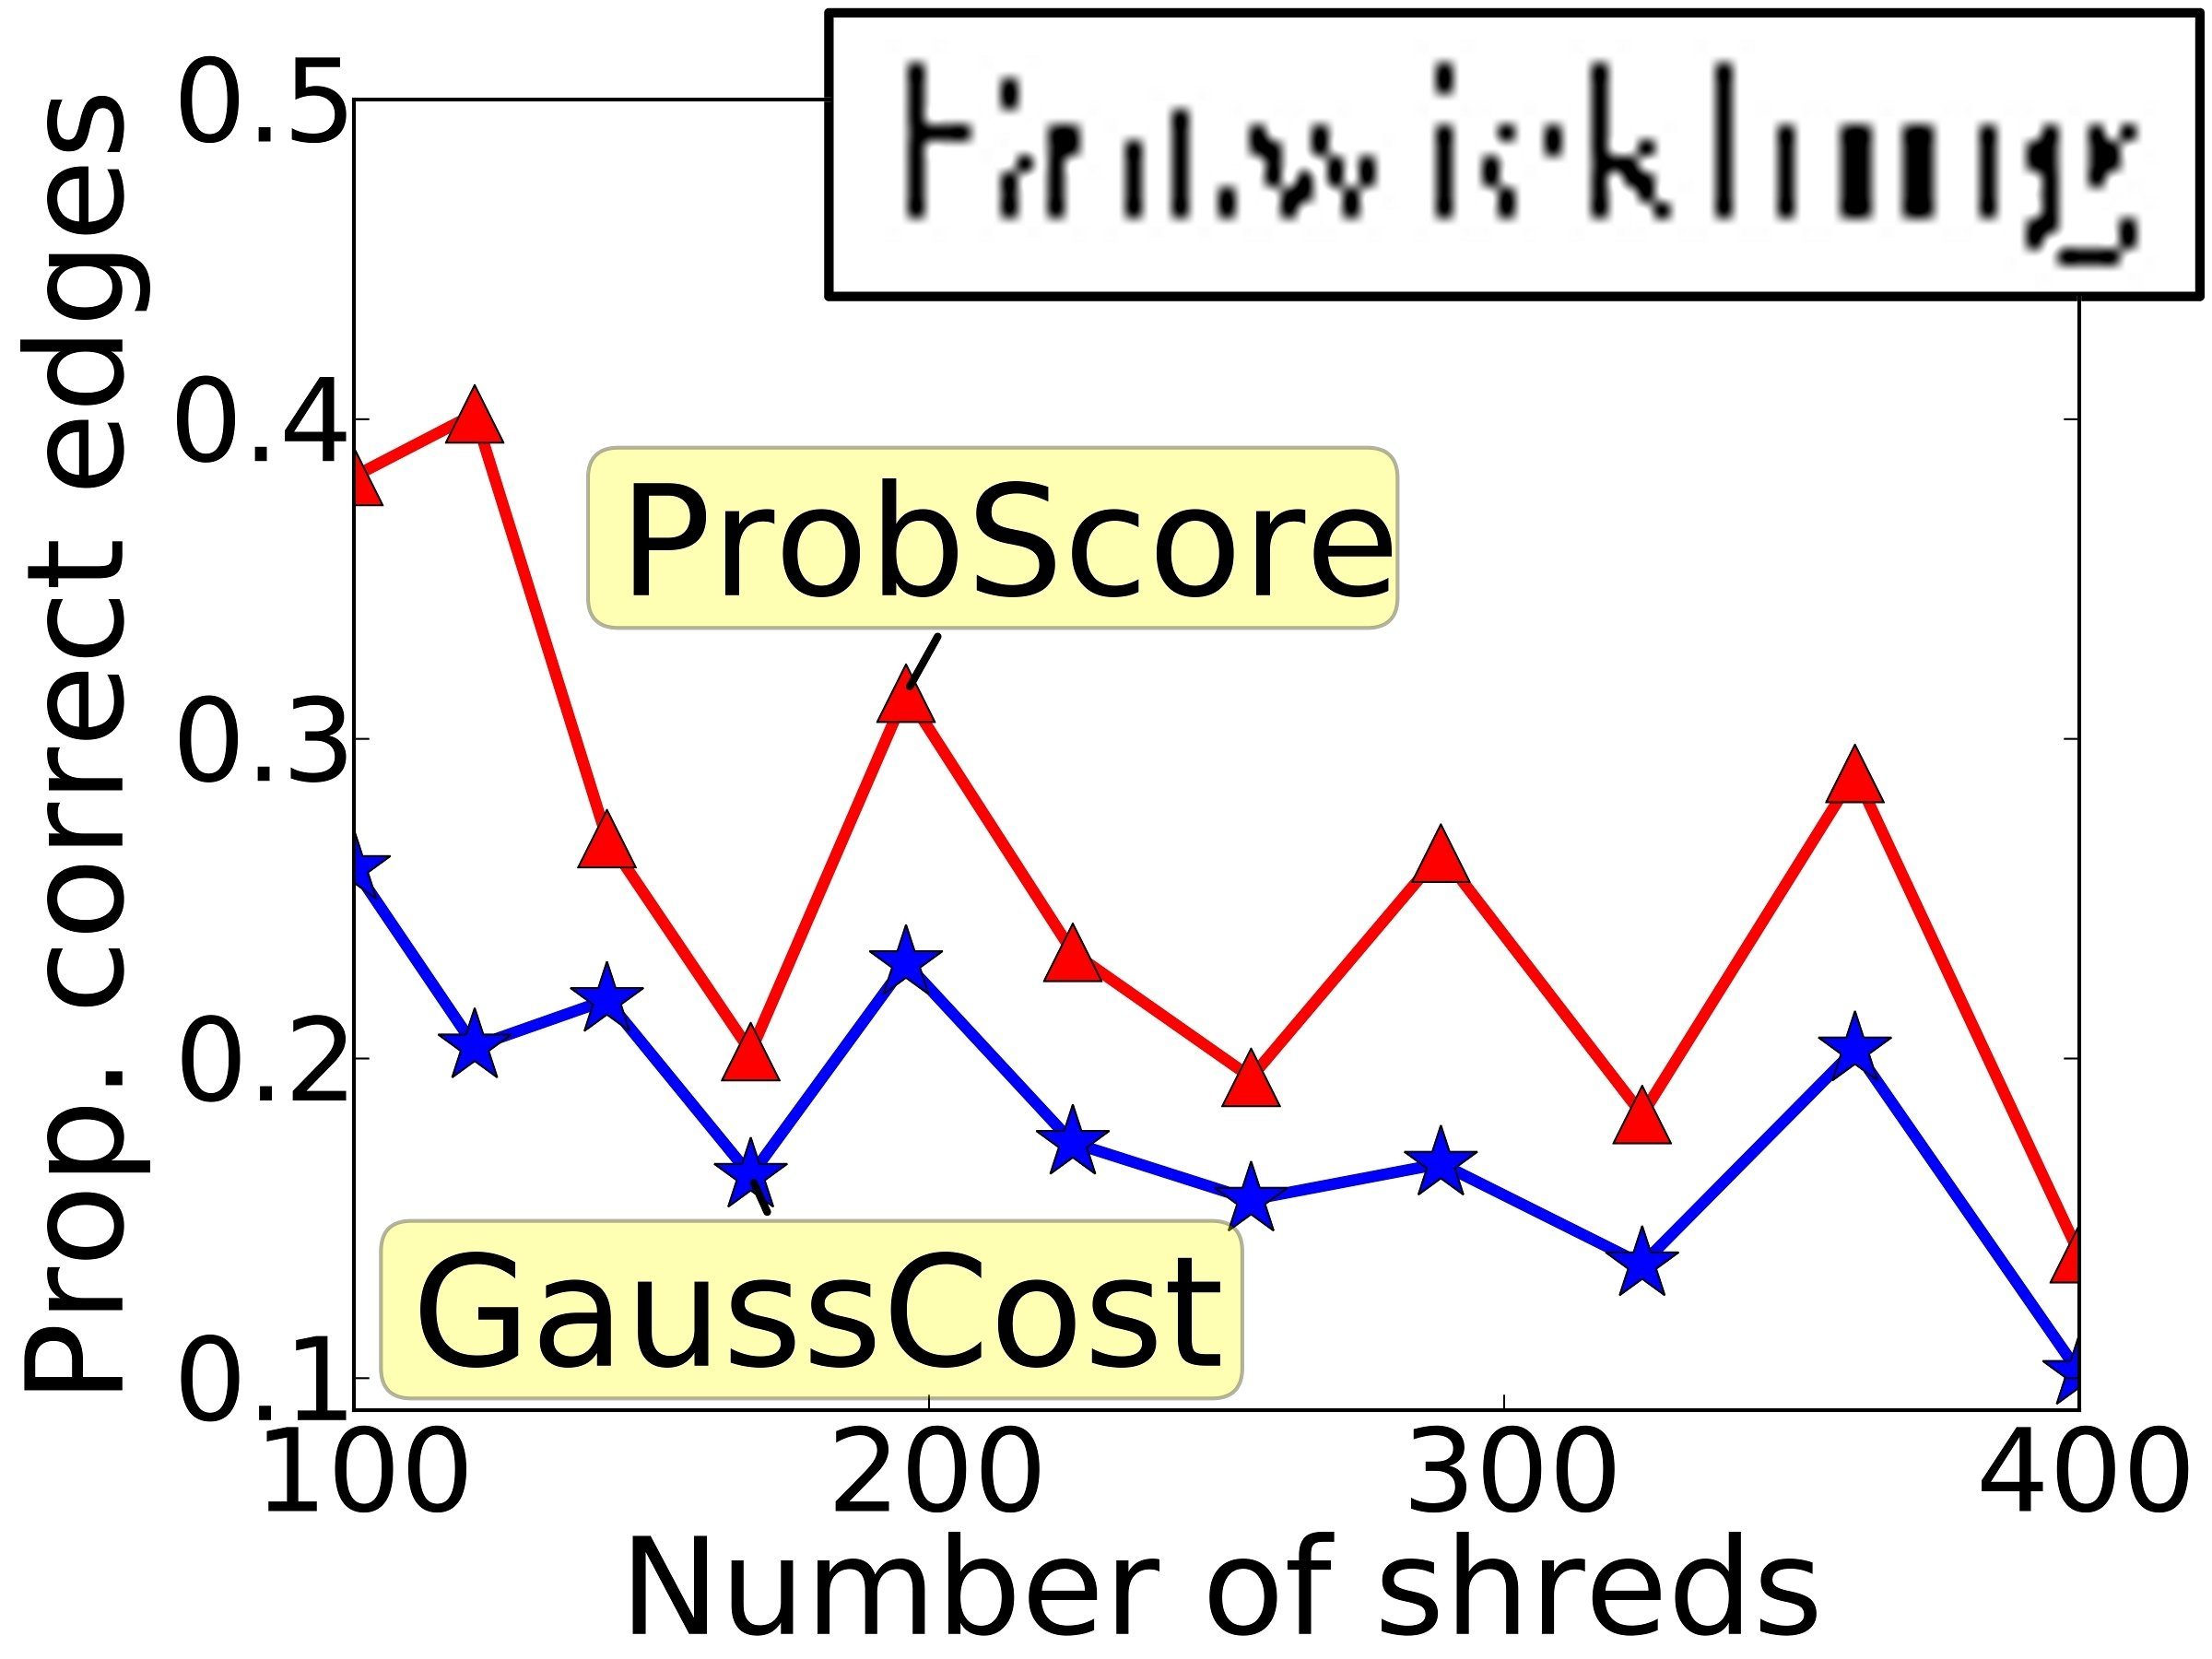
\includegraphics[width=\textwidth]{downsampleCompEnt300.jpg}
        \caption{Downsampled document.}
    \end{subfigure}
    \begin{subfigure}[b]{0.48\textwidth}
        \setlength{\abovecaptionskip}{1pt plus 1.0pt minus 2.0pt}
        \centering
        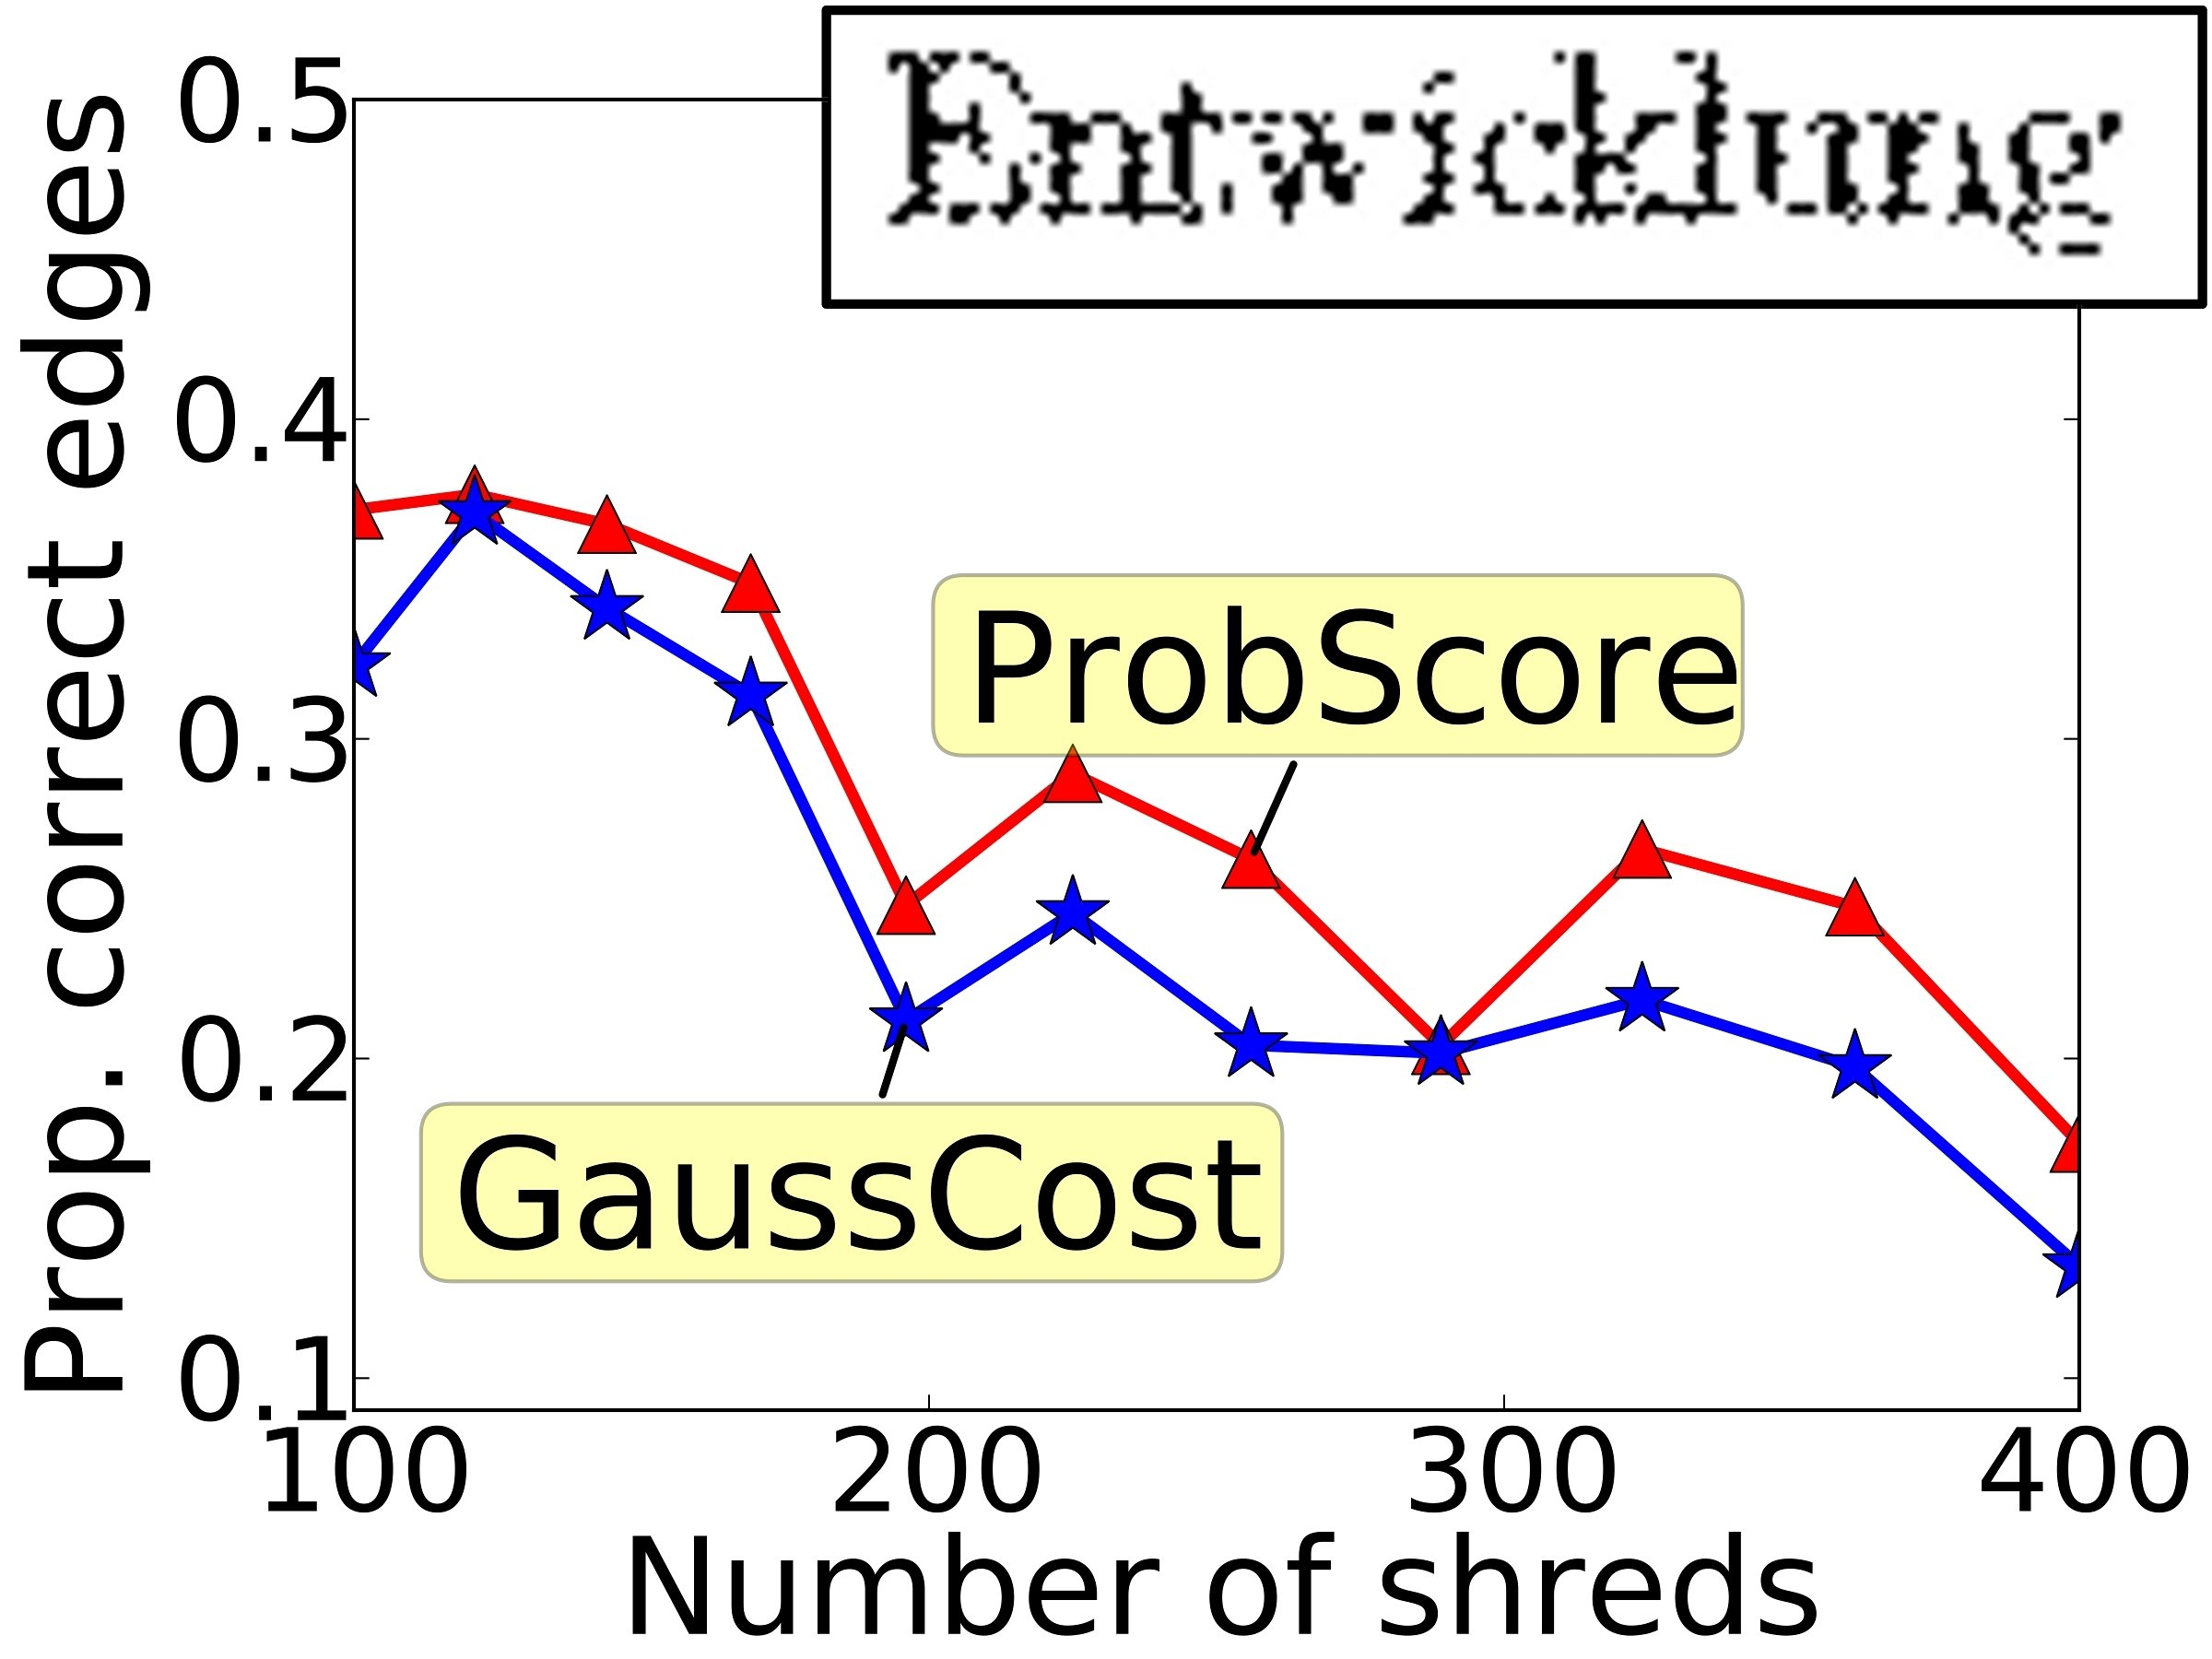
\includegraphics[width=\textwidth]{shuffleCompEnt300.jpg}
        \caption{Noisy document.}
    \end{subfigure}
    \begin{subfigure}[b]{0.48\textwidth}
        \setlength{\abovecaptionskip}{1pt plus 1.0pt minus 2.0pt}
        \centering
        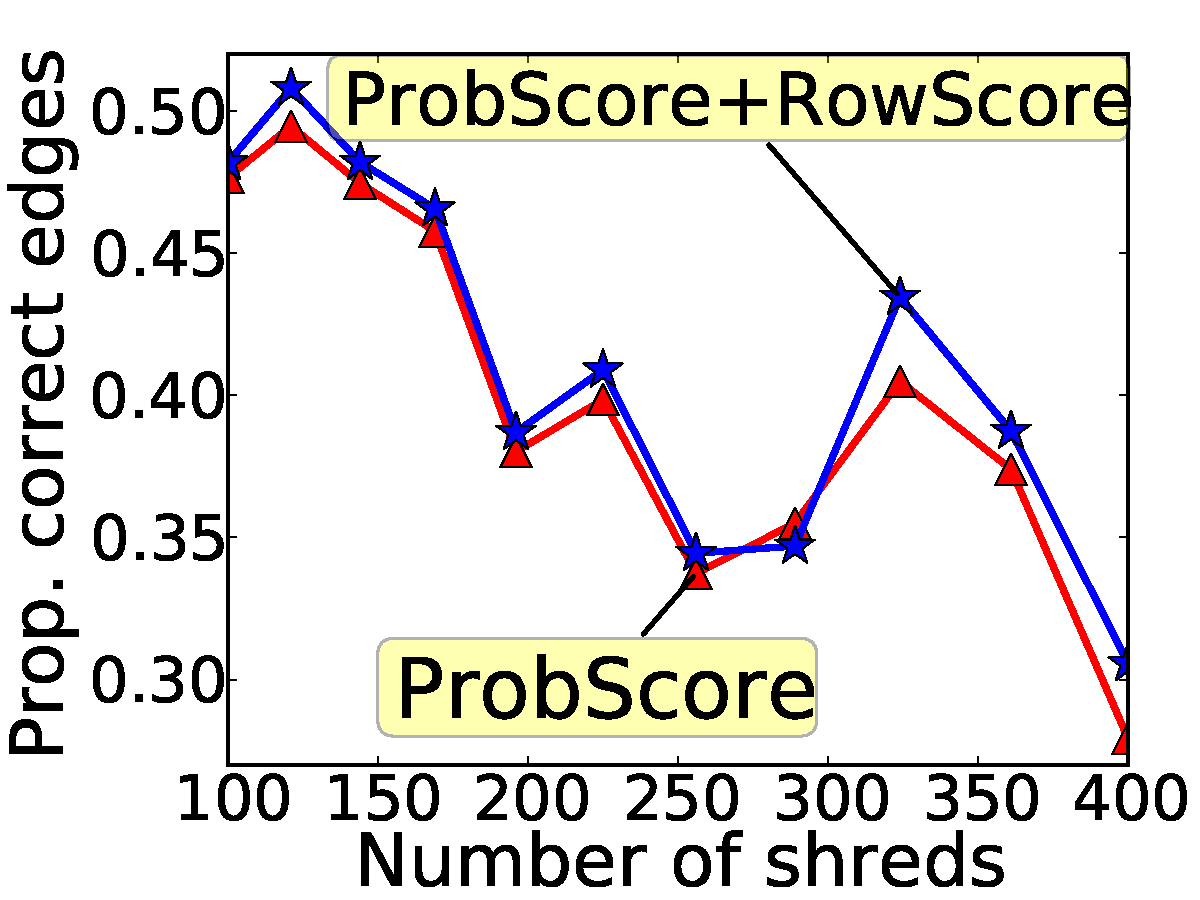
\includegraphics[width=\textwidth]{rowComp.pdf}
        \caption{Score function composition.}
    \end{subfigure}
     \caption{Figures {\bf a}, {\bf b} and {\bf c} compare our method with the most common previously used function. A sample word from each document is shown in the upper right corners. Figure {\bf d} shows the improvement obtained, on a noiseless document, by composing our function with another, very simple, probabilistic model.}
    \label{fig:scoreComp}
\end{figure}

\section{``Kruskal-Inspired" Heuristic Search}
We present a search method inspired by the minimum spanning tree ``Kruskal's algorithm" (\cite{P13}). The method greedily picks the most probable edge and tries to match the two shreds along that edge. This process creates multiple clusters of shreds which will eventually be merged into a single solution. Before performing a merge, we check if the move would result in two shreds being superimposed, in which case the merge is aborted.\footnote{A conceptually similar search heuristic is introduced in \cite{P5}. That formulation, however, uses a static list of scores and thus cannot be used with our probabilistic scoring function which requires the scores to be updated after every merge.} 

The Kruskal heuristic outperforms previously proposed bottom-up heuristics, but is still significantly more tractable\footnote{The Kruskal, Prim and RBH heuristics are written in python, while the ACO, $BV^2$ and $HV^2$ optimisation methods are written in C. Additionally, the implementation of “Kruskal” is a non-optimised proof-of-concept. A non-naive re-implementation could bring its performance more in line to that of “Prim”. As such, the scalability results should be viewed as upper bounds on the performance of the heuristics.}  than any of the top-down optimising search functions (see Figure \ref{fig:searchScal}).

\begin{figure}[h]
    \centering
    \begin{subfigure}[b]{0.48\textwidth}
        \centering
        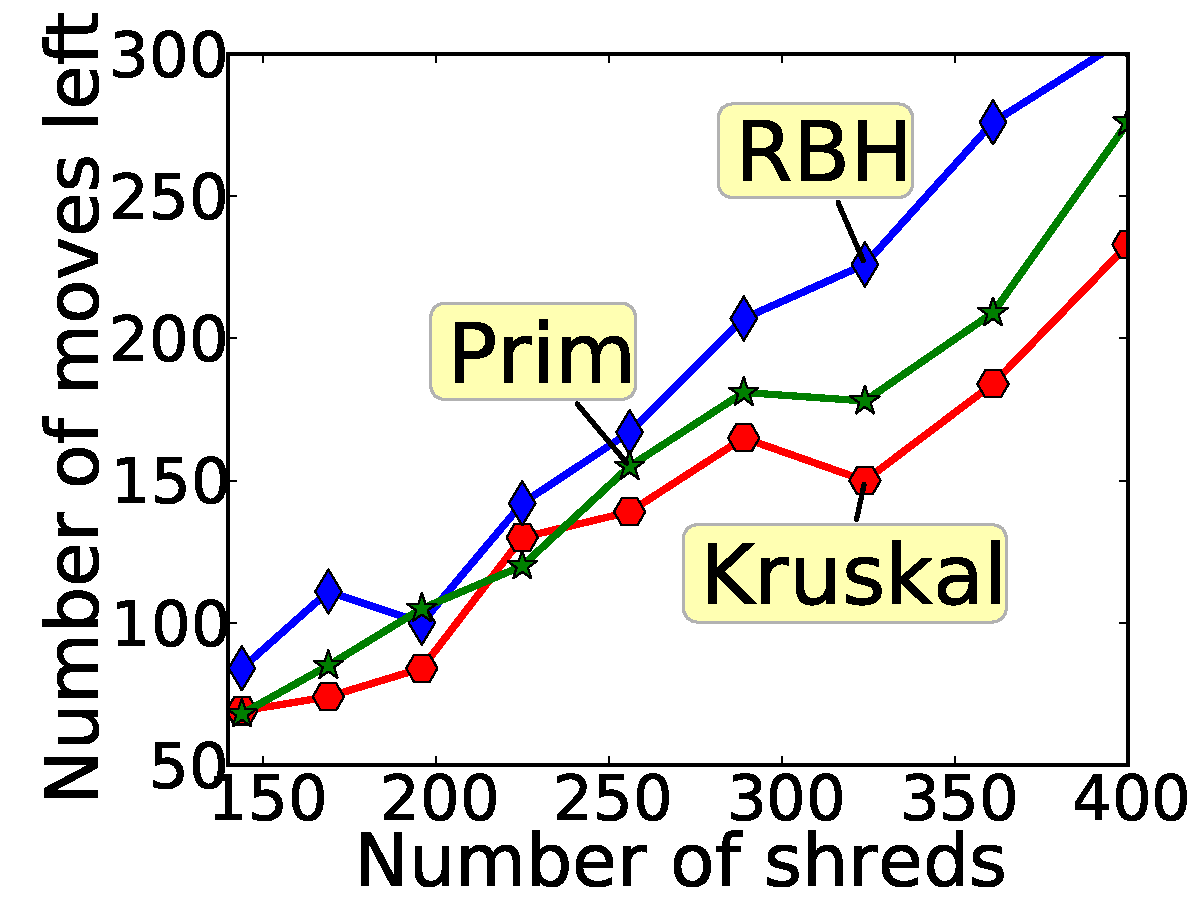
\includegraphics[width=\textwidth]{searchComp.pdf}
        \caption{Performance comparison.}
    \end{subfigure}
    \begin{subfigure}[b]{0.48\textwidth}
        \centering
        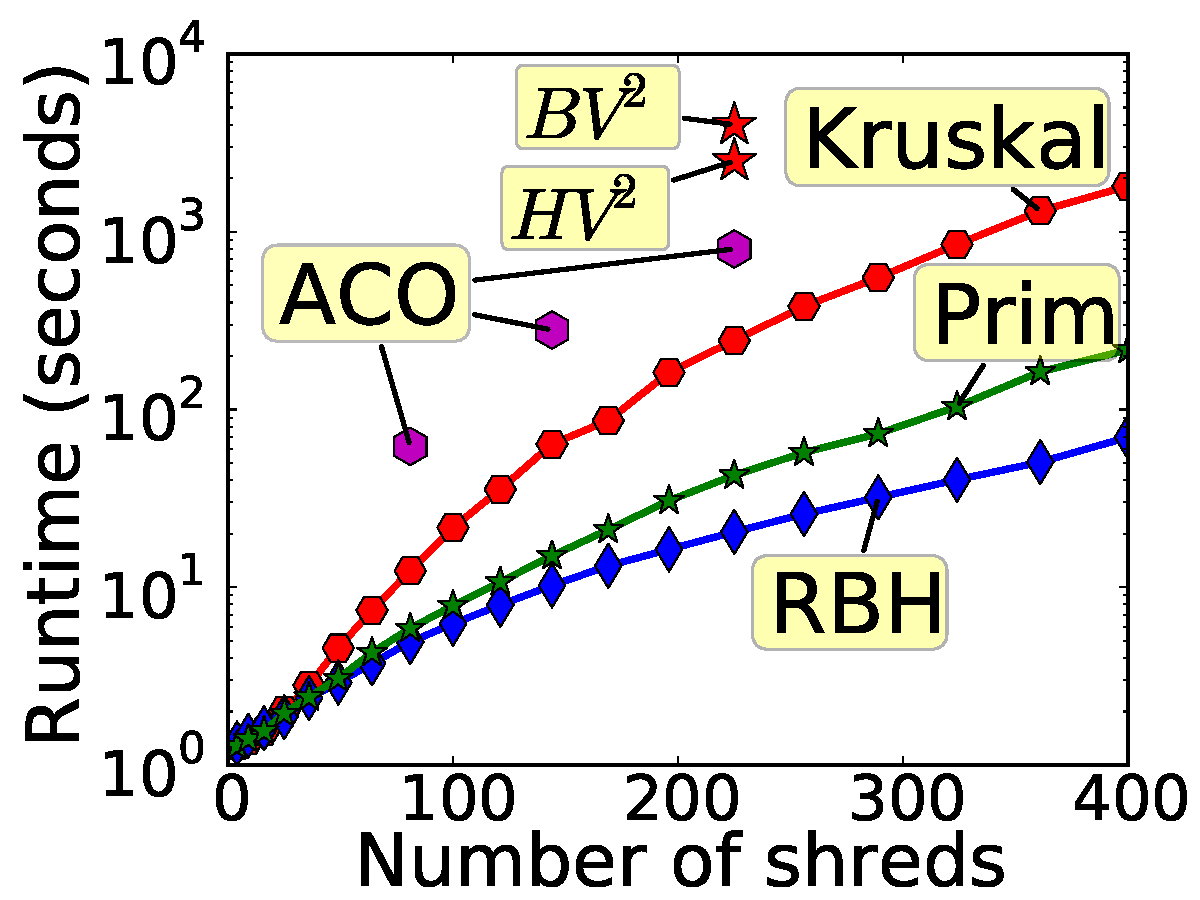
\includegraphics[width=\textwidth]{searchTimeComp.pdf}
        \caption{Runtime comparison.}
    \end{subfigure}
     \caption{Figure {\bf a} shows the performance of our method compared to that of two heuristics introduced in \cite{P3}. Here the X-axis shows how many moves would have to be performed to get from the outputted solution to the correct solution. Figure {\bf b} shows the scalability of our approach when compared to the aforementioned heuristics and a few top down optimising searches introduced in \cite{P4} (ACO is an Ant Colony Optimisation, while $HV^2$ and $BV^2$ are genetic algorithms).}
    \label{fig:searchScal}
\end{figure}

A novel aspect of the Kruskal heuristic is that, if the next move is uncertain, the execution can be stopped. The early stopping mechanism is triggered when the score of the next best move is below some threshold. Once the search has been stopped we return a partial solution, which can significantly reduce the search space of the problem. As seen in Figure \ref{fig:searchReduct}, even the extremely conservative 99.95\% stopping condition helps us reduce the search space to between 40\% and 80\% of its original size.\footnote{A ``99.95\% stopping condition" means that the algorithm continues running only while it is at least 99.95\% sure of the correctness of its next move.} Since the complexity of the search function is exponential in the number of pieces, these reductions are significant and may allow previously intractable search methods to now be run on the smaller instance.

\begin{figure}[t]
    \centering
    \begin{minipage}[b]{0.48\textwidth}
        \centering
        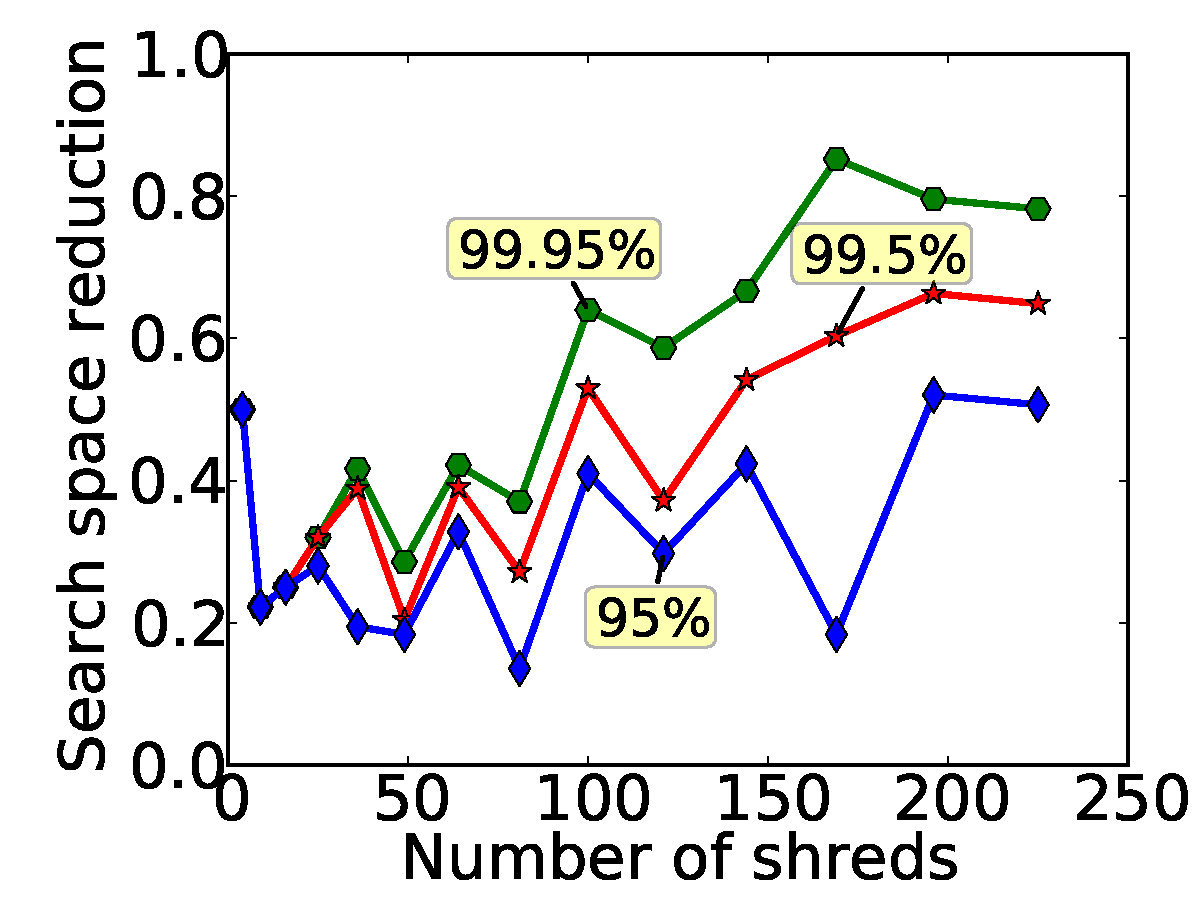
\includegraphics[width=\textwidth]{searchRed.pdf}
        \caption{The reduction in search space corresponding to 3 stopping conditions. ``Search space reduction" is defined as $\frac{\mbox{Final no. pieces}}{\mbox{Initial no. pieces}}$.}
        \label{fig:searchReduct}
    \end{minipage}
    \hfill
    \begin{minipage}[b]{0.48\textwidth}
        \centering
        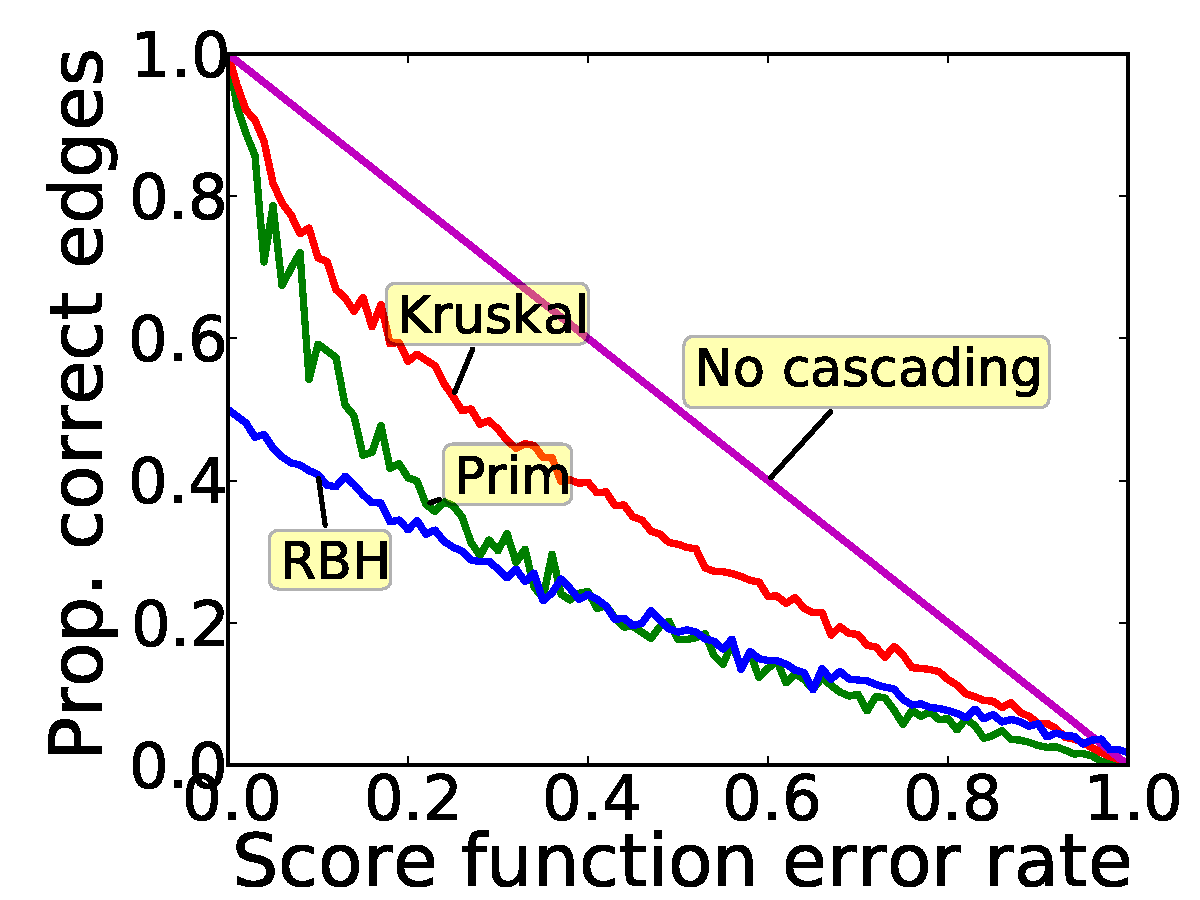
\includegraphics[width=\textwidth]{cascadingComp.pdf}
        \caption{The effect the error in score has on the final error of the method for the 3 search heuristics. The cascading effect causes a small error in the score to be exaggerated by the search method.}
        \label{fig:cascading}
    \end{minipage}
\end{figure}

Another benefit of our Kruskal heuristic can be seen when analysing the \emph{cascading effect}, which is an issue common to all greedy, bottom-up, heuristics. The cascading effect is caused by the inability of the heuristics to correct a wrongly placed shred. This inability means that the search will instead try to find additional pieces which match well with said, wrongly placed, shred. These pieces will therefore have a significant probability of also being wrong, thus starting a chain reaction. While cascading is a problem for all heuristics, our method proves to be more resilient than previous formulations (see Figure \ref{fig:cascading}).

Finally, in Figure \ref{fig:searchRez}, we show some full and partial reconstructions of documents. One thing worth noticing from this example is that cross-cut documents are significantly harder to solve than strip-cut ones, even if the total number of shreds is the same. This difficulty is due to the short edges produced by cross-cutting, which are harder to model accurately. Horizontal cuts also have a significant chance of falling between two lines of text, in which case the score function has no information on how to order the lines.

\begin{figure}[h!]
    \centering
    \begin{subfigure}[b]{\textwidth}
        \centering
        
\includegraphics[width=\textwidth]{prim7x7_300.jpg}
        \caption{Cross-cut document, full solution.}
    \end{subfigure}
    \begin{subfigure}[b]{0.48\textwidth}
        \centering
        
\includegraphics[width=\textwidth]{prim1x49_300.jpg}
        \caption{Strip-cut document, full solution.}
    \end{subfigure}
    \begin{subfigure}[b]{0.48\textwidth}
        \centering
        
\includegraphics[width=0.8\textwidth]{stopped7x7_300.jpg}
        \caption{Cross-cut document, partial solution.}
    \end{subfigure}
     \caption{Figures {\bf a} and {\bf b} show full reconstructions on the cross-cut variant (64\% correct) and the strip-cut variant (100\%correct). Figure {\bf c} shows a partial reconstruction (with a threshold of 99.5\%) which successfully reduces the search space from 49 to 10 shreds while not introducing any errors.}
    \label{fig:searchRez}
\end{figure}

\section{Pre-Processing - Up/Down Orientation Detection}
We present a tractable method for one phase of the pre-processing step, namely the up/down orientation detection of shreds. 
The idea behind this method is to find the \emph{inner} and \emph{outer} rows of each shred, to then count the number of black pixels in the corresponding \emph{upper regions} and \emph{lower regions}, and to finally predict that more black pixels will be present in the upper region (see Figure \ref{fig:rowOrient}). 

In this formulation, we define the outer rows as being delimited by those y coordinates in which a transition is made from a row of pixels that contains no black pixels to a row that contains at least 1 black pixel (or vice versa). We then filter the resulting, preliminary, outer rows such that only those taller than a minimum threshold are kept, since a row that is only 1 or 2 pixels tall is quite likely spurious. Subsequently, we select an inner row inside each outer row by searching for the two y coordinates exhibiting the greatest difference between the sum of black pixels in consecutive rows of pixels. Thus, the greatest increase in number of black pixels between 2 consecutive rows is the upper limit of the inner row, and the greatest decrease is the lower limit of the inner row. 

\begin{figure}[t]
    \setlength{\abovecaptionskip}{4pt plus 1.0pt minus 2.0pt}
    \begin{minipage}[b]{0.44\textwidth}
        \begin{subfigure}[b]{\textwidth}
          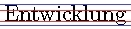
\includegraphics[width=\textwidth]{innerOuterRows300.jpg}
          \caption{The inner lines delimit the inner row, and the outer lines the outer row.}
        \end{subfigure}
        \vspace{1em}

        \begin{subfigure}[b]{\textwidth}
          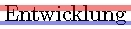
\includegraphics[width=\textwidth]{EntRow300.jpg}
          \caption{For Roman script, the upper region will tend to contain more black pixels than the lower one.}
        \end{subfigure}
     \end{minipage}
      \hfill
    \begin{subfigure}[b]{0.48\textwidth}
        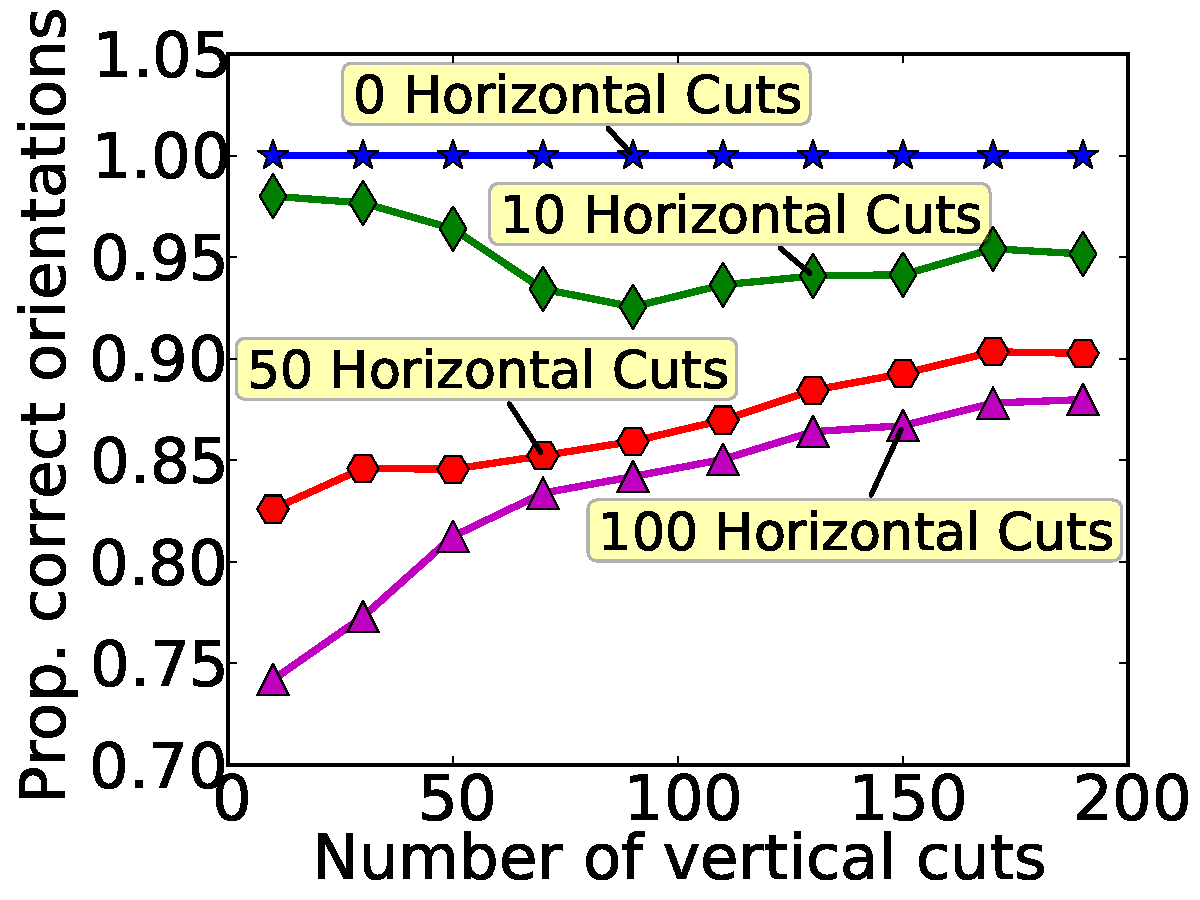
\includegraphics[width=\textwidth]{rowOrient.pdf}
        \caption{The proportion of correctly oriented shreds as the number of cuts grows.}
    \end{subfigure}

     \caption{Figure {\bf a} shows an example of inner and outer rows for one word and Figure {\bf b} shows the corresponding upper and lower regions. Figure {\bf c} shows the results obtained by using these upper and lower regions for orientation detection.}
    \label{fig:rowOrient}
\end{figure}

As can be seen in Figure \ref{fig:rowOrient}, the results are perfect for strip-cut documents (i.e. 0 horizontal cuts) and steadily degrade as we introduce more horizontal cuts. This happens because horizontal cuts reduce the number of rows printed on each shred and therefore make the system more vulnerable to noise. One apparently odd thing about these results is that, for the lower two curves, the performance improves as the number of vertical cuts increases. This behaviour is caused by completely white pieces, which are declared as being always correctly oriented. For the lower two curves, increasing the number of vertical cuts increases the number of white pieces faster than the added noise can degrade the performance, so the overall proportion of correctly predicted orientations increases.

\section{Conclusions and Future Work}
This paper presents a modular and composable framework for the shredded document reconstruction problem and provides sample solutions for several of its components. Specifically, we propose: a probabilistic scoring function which outperforms currently used alternatives; a search heuristic which can either solve simpler reconstruction problems or reduce the search space for more complex ones; and an up/down orientation detection method which obtains good results on taller shreds while being very computationally efficient.

Future work will look at implementing more advanced score and search functions. Solving the cross-cut domain will likely require scoring functions which employ computer vision techniques and search function which solve the cascading problem by performing a partial exploration of the search tree. Additionally, the current state of the pre-processing components makes it necessary to spend a significant amount of time arranging and scanning the shreds, as to minimise noise. Further work is required to create more robust and efficient pre-processing components that will lead to an efficient unshredding pipeline. Lastly the user-interaction aspect needs to be more closely analysed. Good progress has been made by the authors of \cite{P1,P5}, which have shown that a fully automatic reconstruction method can be modified to incorporate user input with relative ease. The question of how to extract the maximum amount of information from a minimum number of user interactions remains, however, open.

\bibliographystyle{plain}
\bibliography{unshredder}
\end{document}
